\section{Theorie}
\label{sec:Theorie}

Der Franck-Hertz Versuch zählt zu den Elektronenstoßexperimenten, mithilfe 
dessen die Struktur von Elektronenhüllen untersucht werden kann. Für dieses 
Experiment wird eine evakuierte Röhre mit Hg-Dampf verwendet. In diesem soll 
es zu sowohl elastischen als auch inelastischen Stößen zwischen Elektronen 
und den Atomen des Hg-Dampfes kommen. Bei diesen Stößen kommt es zu 
Energieunterschieden; Treffen die Elektronen auf ein Atom, kommt es ab einer 
bestimmten Energie zu dem inelastischen Stoß, wobei die Elektronen diskrete 
Energie verlieren und an das Atom abgeben. Dieses ändert folglich sein 
Energieniveau. Diese Energiedifferenz (vor Stoß und nach Stoß) lässt sich 
folgendermaßen kalkulieren:
\begin{align}
    \label{eqn:1}
    \increment E &= E_1 -E_0 \\
                 &= \frac{1}{2} m_0 v_{vor}^2 - \frac{1}{2} m_0 v_{nach}^2.
\end{align}
\noindent $m_0$ sei die Ruhemasse des Elektrons. Die Energien werden mithilfe 
einer Gegenfeldmethode bestimmt, welche im folgenden noch erläutert wird.
Die Atome verweilen jedoch nicht in diesem angeregten Zustand. Stattdessen 
geben sie die gewonnene Energie in Form von emittierten Lichtquanten ab. Die 
Wellenlänge $\lambda$ dieses Lichts beträgt
\begin{equation}
    \label{eqn:lambda}
    \lambda = \frac{ch}{\increment E}.
\end{equation}

\subsection{Idealisierter Franck-Hertz Versuch}
Der schematische Aufbau des Franck-Hertz Versuches befindet sich in \autoref{fig:1}.
\begin{figure}[H]
    \centering
        \centering
        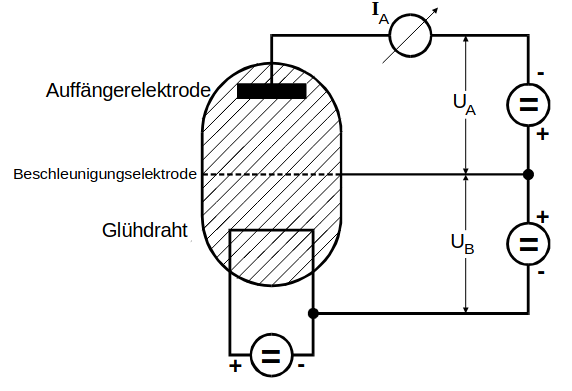
\includegraphics[width=0.65\textwidth]{Bilder/fha.png}
        \caption{Aufbau mit Elementen. \cite{anleitung5}}
    \hfill
    \label{fig:1}
\end{figure}
\noindent In der Röhre befindet sich das erwähnte Quecksilber Gas, welches
teilweise spontan verdampft bis sich ein umgebungstemperaturabhängiger 
Gleichgewichtsdampfdruck einstellt. Folglich lässt sich durch 
die Umgebungstemperatur die Dampfdichte kontrollieren. Jenes ist wichtig für die
Stoßwahrscheinlichkeit, je höher der Druck, desto eher stoßen die Elektronen
mit den Atomen zusammen. Bei zu hohem Druck wiederum würden die Atome gebremst. 
Der Glühdraht sendet durch den glühelektrischen Effekt die Elektronen aus, welche 
diesen umgeben. Die Elektrode in der Mitte der Röhre ist mit einer positiven
Gleichspannung $U_B$ versehen, sie hat den Zweck, die Elektronen zu beschleunigen.
Auf ihrem Beschleunigungsweg beläuft sich die kinetische Energie der Elektronen 
betragsmäßig auf
\begin{align}
    \label{eqn:2}
    E_1 &= E_{Beschleunigung} \\
    \Longleftrightarrow \frac{1}{2} m_0 v_{vor}^2 &= e_0 U_B.
\end{align}
\noindent Am Ende befindet sich die Auffängerlektrode, an welcher der Strom 
$I_A$ liegt. Dieser ist der Auffängerstrom, welcher alle ankommenden Elektronen 
detektiert. Zusätzlich befindet sich hier eine dezente Bremsspannung $U_A$,
welche die Signalqualität verbessern soll, indem sie energiereiche Elektronen 
durchlässt. Dementsprechend wird die anschließende Darstellung der Anregungsenergie 
verbessert. Mathematisch festgehalten schaffen es nur Elektronen an die 
Anode, welche die Ungleichung 
\begin{align}
    \label{eqn:3}
                                    E_{Flucht} &\geq E_{A} \\
    \Longleftrightarrow \frac{1}{2} m_0 v_z ^2 &\geq e_0 U_A
\end{align}
erfüllen. Für die Feststellung, wann das Hg-Atom angeregt wurde, wird $U_B$ 
langsam erhöht. Sobald $U_B \textgreater U_A$, wächst der Elektronenstrom rasant 
an. Wird die Elektronenenergie $\increment E$ überschritten, kommt es zu inelastischen 
Stößen, wobei die Elektronen all ihre Energie bei Stoß übertragen und die 
Auffängerelektrode nicht mehr erreichen, sodass der Auffängerstrom sinkt. 
$U_B$ wird weiter erhöht, damit die Elektronen wieder genügend Energie verfügen 
um bei der Anode anzulangen. Bei erneutem Erreichen der Energie von $\increment E$
kommt es zu inelastischen Stößen und $I_A$ sinkt wie zuvor. Jenes Verfahren 
setzt sich in $U_{1}$-periodischem Abstand fort. Für die Distanz zwischen den 
Maxima gilt der Zusammenhang
\begin{equation}
    \label{eqn:4}
    U_1 = \frac{1}{e_0} \increment E.
\end{equation}
\noindent Jedoch unterliegt der Versuch einigen unvermeidbaren Einflussfaktoren, 
welche im folgenden Kapitel ausgeführt werden.

\subsection{Einflüsse/Störquellen beim Versuch}
\subsubsection{Kontaktpotential}
Aufgrund unterschiedlicher Materlialien der Glühkathode und Beschleunigungselektrode 
liegt eine Potentialdifferenz vor, welche die effektive Beschleunigungsspannung 
verändert. Um ein großes Maß an emittierten Elektronen zu erlangen, wird für 
den Glühdrat ein Material gewählt, dess Austrittsarbeit viel geringer ist als 
die der Beschleunigungselektrode, also: $W_G \textless W_B$. Das dabei 
entstehende Potentialgefälle verursacht eine Verschiebung der Franck-Hertz 
Kurve um das Kontaktpotential K, eine Veranschaulichung liegt in \autoref{fig:1}
vor.
\begin{figure}[H]
    \centering
        \centering
        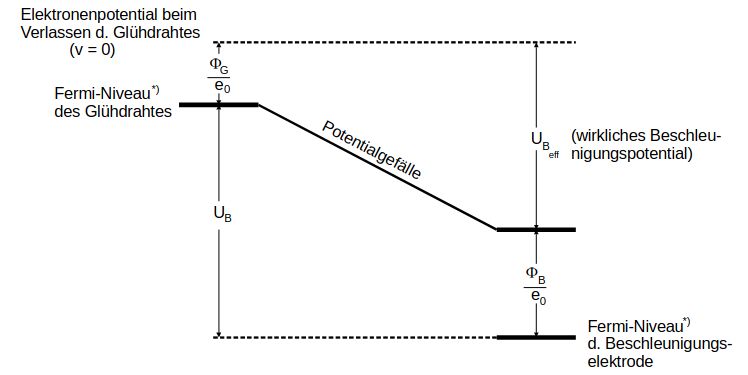
\includegraphics[width=\textwidth]{Bilder/kp.png}
        \caption{Potentialunterschiede. \cite{anleitung5}}
    \hfill
    \label{fig:1}
\end{figure}
\noindent Die Spannung, welche sich letztendlich ergibt, besteht aus der
Beschleuningungsspannungund dem Kontaktpotential.
\begin{align}
    \label{eqn:5}
    U_{B,eff} &= U_B - K \\
              &= U_B - \frac{W_B-W_G}{e_0}
\end{align}

\subsubsection{Energiespektrum der Elektronen}
Die Elektronen sind nach Passieren des Beschleunigungsraums nicht monoenergetisch,
sie werden mit einem kontinuierlichen Spektrum an Energie an der Elektrode 
ausgesendet. Als Folge sinkt $I_A$ nicht auf Null nach Erreichen der Peaks, 
es stellt sich ein Minimum ein.

\subsubsection{Dampfdruck}
Ein weiterer Aspekt ist der Einfluss durch Druck. Der Sättigungsdruck hängt von 
der Temperatur $T$ ab. Folglich verändert sich die Stoßdistanz der Teilchen 
$\overline{w}$ bei Variation der Temperatur, da der Druck dazu führt, dass 
mehr (bei hoher Temperatur) elastische Kollisionen der Elektronen mit den 
Hg-Atomen stattfinden. Wenn nun die Temperatur zu hoch oder zu klein ist, 
treten dementsprechend viele elastische Stöße auf, wodurch das Hg-Atom 
nicht angeregt wird, da die Elektronen keine Zeit haben genügend Energie 
aufzunehmen oder sie fliegen ungebremst durch das Feld, da es zu keinen 
Kollisionen kommt. Es gilt als Zusammenhang
\begin{equation}
    \label{eqn:6}
    \overline{w} = 5.5 \cdot 10^7 \exp \left(-\frac{6876}{T} \right).
\end{equation}
\noindent Dabei sei die mittlere freie Weglänge angegeben in $\unit{\centi\meter}$.

\subsection{Fehlerrechnung}
Die gemessenen Werte unterliegen Messunsicherheiten und werden demnach im
Folgenden nicht als fehlerfrei angesehen. Die Fehler entstehen bei der
Bildung der Mittelwerte durch den Fehler des Mittelwerts und bei der
Regressionsrechnung sowie der Fehlerforpflanzung durch Python.
Der Fehler des Mittelwerts ist gegeben durch 
\begin{equation}
    \begin{aligned}
        \increment \overline{x} &= \sqrt{\overline{x^2\kern-0.1em} - \overline{x}^2} \\
                            &= \frac{\sqrt{\frac{1}{N-1} \sum\limits_{i=1}^N (x_i - \overline{x})^2}}{\sqrt{N}}.
    \end{aligned}
\end{equation}

Um Fehler einzubeziehen, wird die Gauß'sche Fehlerfortpflanzung verwendet:
\begin{equation}
    \label{eqn:9}
    \increment f = \sqrt{\left(\frac{\partial f}{\partial x}\right)^2 \cdot \left(\increment x\right)^2 + \left(\frac{\partial f}{\partial y}\right)^2 \cdot \left(\increment y\right)^2 + .... + \left(\frac{\partial f}{\partial z}\right)^2 \cdot \left(\increment z\right)^2}
\end{equation}